\documentclass[10pt]{article}

\usepackage[utf8]{inputenc}
\usepackage[french]{babel}
\usepackage{amsmath}
\usepackage{amsfonts}
\usepackage{amssymb}
\usepackage{graphicx}
\usepackage{parskip}
\usepackage{multicol}


\newcommand{\NP}{\text{NP}}

\begin{document}


\title{IFT2105 - Devoir 3}
\date{Novembre 2010}
\author{Vincent Foley-Bourgon (FOLV08078309)}
\maketitle

\section{Question 1}

\emph{Montrer que L est NP-complet où:}
\[
L = \{ G : G \text{ est un graphe de $n$ noeuds ayant une clique de
  taille au moins $n/2$} \}
\]

Le langage $L$ est NP-complet si:
\begin{enumerate}
  \item $L \in \NP$
  \item $L$ est NP-difficile
\end{enumerate}

\subsection{$L \in \NP$}

$L$ appartient à la classe NP s'il existe une machine de Turing
fonctionnant en temps polynomial qui, étant donné un certificat $C$,
\emph{vérifie} si un mot appartient à $L$.

Prenons comme certificat l'ensemble des noeuds formant la clique; il
est possible de vérifier en temps polynomial que ces noeuds forment un
graphe complet:

\begin{verbatim}
Verificateur(G, C):
  si |G|/2 > |C|:
    retourner faux

  pour chaque noeud dans C:
    pour chaque autre-noeud dans C \ {noeud}:
      si noeud et autre-noeud ne sont pas voisins:
        retourner faux

  // Tous les noeuds sont voisins
  retourner vrai
fin
\end{verbatim}

\emph{Verificateur} fonctionne en $O(n^2)$, donc $L \in \NP$.

\subsection{$L$ est NP-difficile}

$L$ est NP-difficile si $L$ est au moins aussi difficile que tous les
autres langages dans NP.  Écrit de façon mathématique, pour tout
langage $K$ de NP, il existe une machine de Turing qui permet de
réduire $K$ à $L$ en temps polynomial (noté $K \le_p L$) et où $w
\in K \iff f(w) \in L$.

\subsubsection{Fonction de réduction}

Nous savons que le langage CLIQUE est NP-complet.  Voici sa
définition:

\[
\text{CLIQUE} = \{ \langle G, k \rangle : G \text{ possède un sous-graphe complet de
  $k$ sommets} \}
\]


Cherchons une fonction de réduction de CLIQUE vers $L$ qui s'exécute
en temps polynomial.

Nous allons faire une fonction qui:

\begin{enumerate}
\item Crée un graphe $G_2$ contenant le même nombre de sommets que $G$
\item Crée une clique de $|G|-k$ sommets dans $G_2$.
\item Connecte tous les sommets de $G$ à tous les sommets de $G_2$
  (formant ainsi un graphe que nous appelerons $G_t$, $t$ pour total).
\end{enumerate}

\begin{verbatim}
Reduction(G, k):
  G2 = nouveau Graphe

  // 1
  pour i = 1 à |G|:
    G2.AjouterSommet(i)

  // 2
  pour i = 1 à |G|-k
    pour j = i à |G|-k
      Connecter(G2[i], G2[j])

  // 3
  pour chaque sommet s1 de G:
    pour chaque sommet s2 de G:
      Connecter(s1, s2)
fin
\end{verbatim}

L'étape 1 s'exécute en $O(n)$, l'étape 2 s'exécute en $O(n^2)$ et
l'étape 3 s'exécute en $O(n^2)$.  La somme de 3 polynômes est un
polynôme, donc la fonction de réduction s'exécute en temps polynomial.



\subsubsection{$\langle G,k \rangle \in \text{CLIQUE} \implies Reduction(\langle G,k \rangle) \in L$}

\begin{itemize}
\item En joignant $G$ et $G_2$, on a que $|G_t| = |G| + |G_2| = 2|G|$.
\item $G$ contient une $k$-clique.
\item $G_2$ contient une $(|G|-k)$-clique.
\item En joignant tout les sommets de $G$ à ceux de $G_2$, on a joint
  tous les sommets formant les deux cliques ensemble, donc $G_t$
  contient une clique de taille $k + (|G|-k) = |G| = |G_t|/2$.
\end{itemize}

Et donc, si $\langle G,k \rangle$ appartient à CLIQUE, alors
$Reduction(\langle G,k \rangle)$ appartient à notre langage $L$.


\subsubsection{$\langle G,k \rangle \not\in \text{CLIQUE} \implies
  Reduction(\langle G,k \rangle) \not\in L$ (contraposée)}

\begin{itemize}
\item En joignant $G$ et $G_2$, on a que $|G_t| = |G| + |G_2| = 2|G|$.
\item $G$ ne contient \textbf{pas} une $k$-clique.
\item $G_2$ contient une $(|G|-k)$-clique.
\item En joignant tout les sommets de $G$ à ceux de $G_2$, la clique
  maximale pouvant se trouver dans $G_t$ a une taille strictement
  inférieure à $k + (|G|-k) = |G| = |G_t|/2$.
\end{itemize}

Et donc, si $\langle G,k \rangle$ ne contient \textbf{pas} une
$k$-clique, alors $Reduction(\langle G,k \rangle)$ n'appartient pas à
notre langage $L$.

\subsection{Conclusion}

Comme nous avons démontré que $L \in NP$ et que $L$ est NP-difficile,
nous avons donc démontré que $L$ est un langage NP-complet.

\newpage

\section{Question 2}

\emph{Montrer que L est NP-complet où:}
\[
L = \{ \langle C_1, C_2 \rangle : \text{$C_1$ et $C_2$ calculent une
  fonction différente} \}
\]

Le langage $L$ est NP-complet si:
\begin{enumerate}
  \item $L \in \NP$
  \item $L$ est NP-difficile
\end{enumerate}

\subsection{$L \in \NP$}

$L$ appartient à NP s'il existe une machine de Turing qui le vérifie
en temps polynomial.

\begin{verbatim}
Verificateur(C1, C2, C):
  retourner C1(C) != C2(C)
fin
\end{verbatim}

\emph{Verificateur} exécute les deux circuits booléens avec le
certificat (la valeur des différentes variables booléennes) et
retourne vrai si $C_1$ et $C_2$ calculent un résultat différent et
faux s'ils calculent le même résultat.  L'exécution de $C_1$ et de
$C_2$ se fait en temps polynomial, donc l'exécution de
\emph{Verificateur} se fait aussi en temps polynomial, et donc $L \in
\NP$.

\subsection{$L$ est NP-difficile}

$L$ est NP-difficile si tous les langages $L'$ dans NP peuvent se
réduire à $L$ en temps polynomial et si $w \in L' \iff f(w) \in L$.

\subsubsection{Fonction de réduction}

Utilisons le langage NP 3-SAT pour montrer que $L$ est NP-complet.
Nous allons réduire une expression $\phi \in \text{3-SAT}$ à $L$ comme
ceci:

\begin{verbatim}
Reduction(phi):
  C1 = Construire le circuit booléen associé à phi
  C2 = Construire le circuit booléen associé à (phi et 0)
  retourner <C1, C2>
fin
\end{verbatim}

La construction d'un circuit booléen à partir d'une expression
booléenne se fait en temps polynomial, et la somme de deux polynômes
et un polynôme, donc \emph{Reduction} fonctionne en temps polynomial.

\subsubsection{$\phi \in \text{3-SAT} \implies Reduction(\phi) \in L$}

\begin{itemize}
\item $\phi$ est dans 3-SAT, donc $\phi = 1$
\item $\phi \wedge 0 = 1 \wedge 0 = 0$
\item Les circuits $C_1$ et $C_2$ associés à $\phi$ et $(\phi \wedge 0)$
  calculent des résultats différents.
\end{itemize}

Donc, si $\phi$ est dans 3-SAT, alors $Reduction(\phi)$ est dans notre
langage $L$.


\subsubsection{$\phi \not\in \text{3-SAT} \implies Reduction(\phi)
  \not\in L$ (contraposée)}

\begin{itemize}
\item $\phi$ n'est \textbf{pas} dans 3-SAT, donc $\phi = 0$
\item $\phi \wedge 0 = 0 \wedge 0 = 0$
\item Les circuits $C_1$ et $C_2$ associés à $\phi$ et $(\phi \wedge 0)$
  calculent des résultats égaux.
\end{itemize}

Donc, si $\phi$ n'est \emph{pas} dans 3-SAT, alors $Reduction(\phi)$
n'est pas dans notre langage $L$.

\subsection{Conclusion}

Comme $L$ appartient à NP et qu'il est NP-difficile, alors $L$ est NP-complet.

\newpage

\section{Question 3}

\emph{Montrer que pour tout $k$ fixe, $k$-CLIQUE est dans P.}

Un langage $L$ est dans P s'il existe une machine de Turing
fonctionnant en temps polynomial qui \emph{décide} si un mot $w$
appartient au langage.

Pour démontrer que pour un $k$ fixe, $k$-CLIQUE est dans P, il suffit
de donner un algorithme polynomial qui décide si un graphe possède une
clique de taille $k$.

Considérons le graphe $G$ suivant:

\begin{figure}[h]
  \centering
  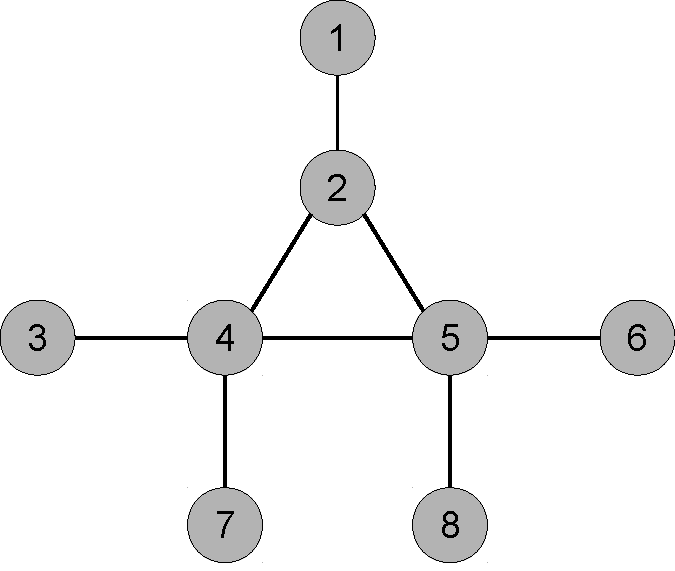
\includegraphics[scale=0.4]{graphe3}
\end{figure}

et définissons un algorithme pour déterminer s'il possède une
3-CLIQUE:

\begin{verbatim}
Possede-Une-3Clique(G):
  pour i := 1 à |G|-2:
    pour j := i+1 à |G|-1:
      pour k := j+1 à |G|:
        si (i, j, k) sont tous voisins:
          retourner vrai

  // Aucune 3-clique n'a été trouvée
  retourner faux
fin
\end{verbatim}

L'algorithme trouvera qu'il existe une 3-CLIQUE entre les noeuds 2, 4
et 5.

Cet algorithme fonctionne en $O(n^3)$, clairement un temps polynomial.
Pour décider si un graphe possède une 4-CLIQUE, on ajouterait une
quatrième boucle dans le corps de l'algorithme et le temps d'exécution
serait $O(n^4)$.  Un algorithme décidant si un graphe possède une
$k$-CLIQUE pour un $k$ fixe fonctionnerait en $O(n^k)$, un temps
polynomial.

Donc, pour un $k$ fixe, décider si un graphe appartient à $k$-CLIQUE
se fait en temps polynomial, et ce langage appartient à P.


\end{document}






